
Las funciones son bloques de código reutilizables que realizan una tarea específica. Permiten dividir un programa en partes más pequeñas y manejables, lo que facilita la comprensión y el mantenimiento del código. La modularidad se refiere a la práctica de dividir un programa en módulos o funciones independientes que pueden ser desarrolladas y probadas de forma separada. Esto promueve el código limpio y organizado, facilitando la colaboración en equipos de desarrollo.

\subsection{Definición y llamada de funciones}

Definición de Funciones:\\
  
En la mayoría de los lenguajes de programación, las funciones se definen con la palabra clave ``def'' (en Python), ``function'' (en JavaScript), ``fun'' (en Kotlin), o ``void'' (en C++), seguido del nombre de la función y una lista de parámetros entre paréntesis. Por ejemplo, en Python:
\begin{figure}[h]
    \centering
    \scalebox{0.35}{
    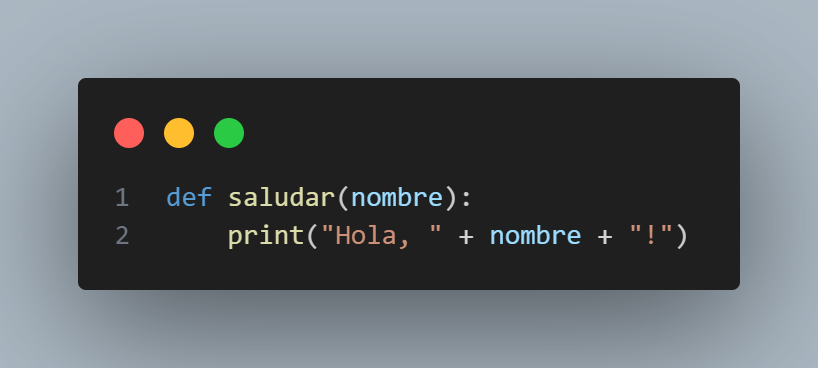
\includegraphics{Imagenes/funciones1.png}
    }
  \end{figure}

Llamada de Funciones:\\

Para utilizar una función, se realiza una llamada a la función, pasando los valores necesarios como argumentos. Los argumentos son los valores reales que se pasan a la función durante la llamada. Por ejemplo:

\begin{figure}[h]
    \centering
    \scalebox{0.35}{
    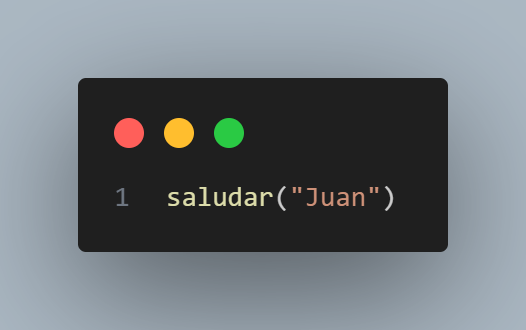
\includegraphics{Imagenes/funciones2.png}
    }
  \end{figure}

En este caso, ``Juan'' es el argumento que se pasa a la función ``saludar''.

\subsection{Argumentos y parámetros}
Parámetros de Funciones:\\

Los parámetros son variables que se utilizan en la definición de la función para aceptar valores. En el ejemplo anterior, ``nombre'' es un parámetro de la función ``saludar''.
\begin{figure}[h]
    \centering
    \scalebox{0.35}{
    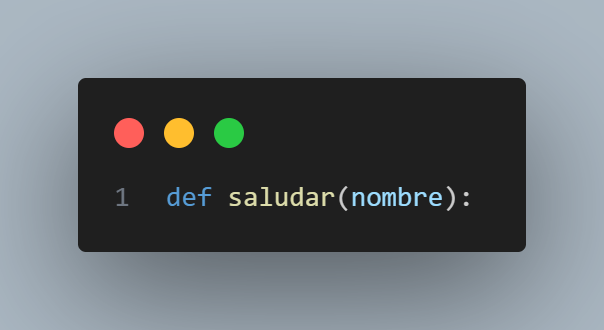
\includegraphics{Imagenes/funciones3.png}
    }
  \end{figure}

Argumentos de Funciones:\\

Los argumentos son los valores reales que se pasan a la función durante su llamada. En el ejemplo de la llamada a la función `saludar("Juan")`, "Juan" es el argumento que se pasa al parámetro ``nombre'' de la función ``saludar''\\

Las funciones pueden tener múltiples parámetros y se pueden pasar argumentos de diferentes tipos (números, cadenas, listas, etc.). Por ejemplo:

\begin{figure}[h]
    \centering
    \scalebox{0.35}{
    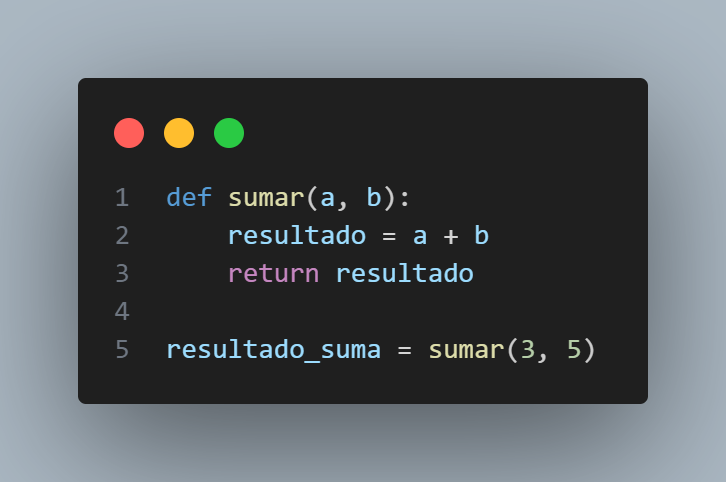
\includegraphics{Imagenes/funciones4.png}
    }
  \end{figure}

En este caso, la función ``sumar'' tiene dos parámetros ``a'' y ``b'', y se llama con los argumentos 3 y 5, respectivamente. El resultado de la suma se almacena en la variable ``resultado\_suma''.\\

Las funciones y la modularidad son conceptos fundamentales en programación, ya que permiten escribir código más eficiente, fácil de entender y mantener. La práctica constante con estos conceptos te ayudará a mejorar tus habilidades de programación.

\subsection{Módulos y su importación}
Los módulos son archivos que contienen definiciones y declaraciones de funciones, clases y variables en Python. Ayudan a organizar el código en archivos separados para hacerlo más legible y reutilizable. Para utilizar las funciones y variables definidas en un módulo en otro archivo, se necesita importar el módulo en el archivo donde se desea utilizar.

\begin{itemize}
    \item Creación de un Módulo: Supongamos que tenemos un archivo llamado mi\_modulo.py con la siguiente definición de función:
    \begin{figure}[h]
        \centering
        \scalebox{0.35}{
        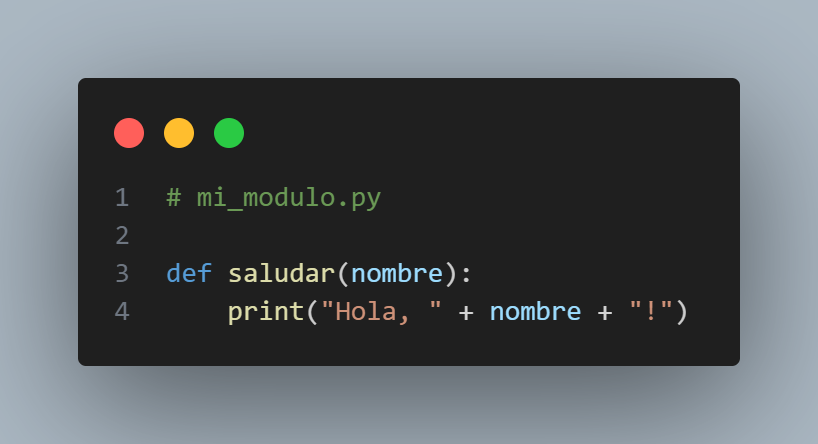
\includegraphics{Imagenes/funciones5.png}
        }
      \end{figure}

    \item Importación de un Módulo: En otro archivo Python, podemos importar y utilizar la función saludar del módulo mi\_modulo.py de la siguiente manera:
    \begin{figure}[h]
        \centering
        \scalebox{0.35}{
        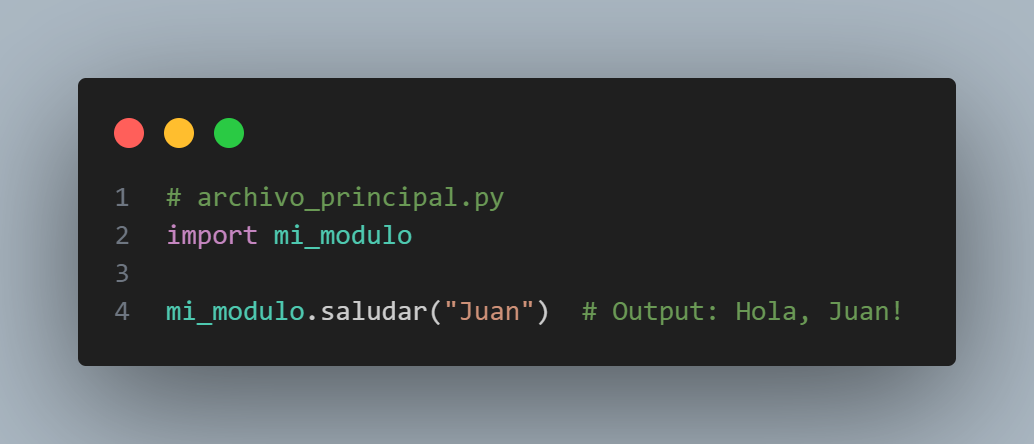
\includegraphics{Imagenes/funciones6.png}
        }
      \end{figure}
      
      También se puede importar una función específica de un módulo para evitar usar el nombre del módulo cada vez que se llama a la función:

      \begin{figure}[h]
        \centering
        \scalebox{0.35}{
        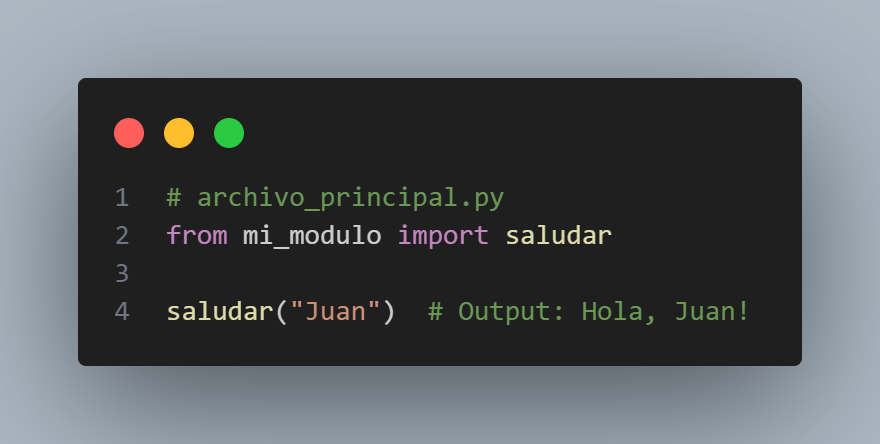
\includegraphics{Imagenes/funciones7.png}
        }
      \end{figure}
    \end{itemize}
      
    La importación de módulos es esencial para organizar proyectos grandes y complejos en Python, ya que permite dividir el código en archivos manejables y fácilmente comprensibles. Además, facilita la reutilización del código, ya que las funciones y variables definidas en un módulo pueden ser utilizadas en varios archivos del proyecto.


